\documentclass[a4paper,10pt]{article}
\usepackage[utf8]{inputenc}
\usepackage{graphicx}
\usepackage{amsmath}
\usepackage{amssymb}
\usepackage{epstopdf}
\usepackage{bm}
\usepackage{hyperref}
\usepackage{amsthm}
\usepackage{caption}
\usepackage{tikz}
% 
% 
\title{Dirichlet-Neumann Iteration}
\begin{document}
\maketitle
% 
\section{Continuous version}
% 
\begin{center}
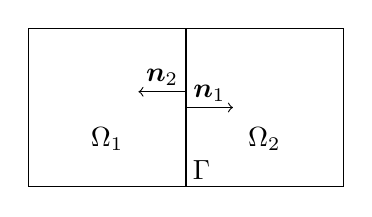
\begin{tikzpicture}[scale = 2]
\draw [-] (1,1) -- (3,1) -- (3,2) -- (1,2) -- (1,1);
\draw [-, thick] (2,1) -- (2,2);
 
\node at (1.5, 1.3) {$\Omega_1$};
\node at (2.5, 1.3) {$\Omega_2$};

\draw [->] (2,1.5) -- (2.3, 1.5); \node at (2.15, 1.59) {$\bm{n}_1$};
\draw [->] (2,1.6) -- (1.7, 1.6); \node at (1.85, 1.69) {$\bm{n}_2$};
\node at (2.1, 1.1) {$\Gamma$};
\end{tikzpicture}
\end{center}
% 
Base Problem: Poisson equation (stationary heat equation, think $t\rightarrow \infty$)
% 
\begin{align}\label{EQ PDE}
\begin{split}
\Delta u (x, y) &= 0, \quad (x, y) \in \Omega = \Omega_1 \cup \Omega_2 \\
u(x, y) &= g(x, y), \quad (x, y) \in \partial \Omega
\end{split}
\end{align}
% 
Here, $\partial \Omega$ is the boundary of $\Omega$ and $g(x, y)$ is the prescribed (Dirichlet) boundary condition.

Now, consider $u(x, y)$ split into $u_1(x, y)$ and $u_2(x, y)$, according to their respective domains $\Omega_1$ and $\Omega_2$

Then, we add the following redundant conditions to the above PDE:
%
\begin{align}
\nabla u_1 (x, y) \cdot \bm{n}_1 &= -\nabla u_2 (x, y) \cdot \bm{n}_2, \quad (x, y) \in \Gamma, \label{EQ FLUX COND}\\
u_1 (x, y) & = u_2 (x, y), \quad (x, y) \in \Gamma. \label{EQ CONT COND}
\end{align}
% 
That is, the solution and its derivative are continuous at $\Gamma$.

The domain decomposition approach is to solve the PDE, here the Poisson equation \eqref{EQ PDE}, on subdomains. That is, we solve \eqref{EQ PDE} on $\Omega_1$ and $\Omega_2$ separately. Now, we lack a boundary condition at $\Gamma$. The solution is to enforce \eqref{EQ CONT COND} for the problem corresponding to $\Omega_1$ and \eqref{EQ FLUX COND} for the problem corresponding to $\Omega_2$.

The iteration is then as follows: Given an initial guess $u_\Gamma^{(0)}$, solve
% 
\begin{align}
\begin{split}
\Delta u_1^{(k+1)} (x, y) &= 0, \quad (x, y) \in \Omega_1,\\
u^{(k+1)}_1(x, y) &= g(x, y), \quad (x, y) \in \partial \Omega_1\setminus \Gamma, \\
u^{(k+1)}_1(x, y) & = u_\Gamma^{(k)}, \quad (x,y) \in \Gamma,
\end{split}
\end{align}
% 
i.e., given a Dirichlet boundary condition at $\Gamma$, solve the Poisson equation on $\Omega_1$. Based on the solution $u_1^{(k+1)}(x,y)$, we can compute the heat flux $q_\Gamma^{(k+1)}(x, y) = -\nabla u_1 (x, y) \cdot \bm{n}_1$. Using this, we can solve the problem on $\Omega_2$, using the heat flux $q_\Gamma^{(k+1)}(x, y)$ as boundary condition:
% 
\begin{align}
\begin{split}
\Delta u_2^{(k+1)} (x, y) &= 0, \quad (x, y) \in \Omega_2,\\
u^{(k+1)}_2(x, y) &= g(x, y), \quad (x, y) \in \partial \Omega_2\setminus \Gamma, \\
\nabla u^{(k+1)}_2(x, y) \cdot \bm{n}_2 & = q_\Gamma^{(k+1)}(x, y), \quad (x,y) \in \Gamma.
\end{split}
\end{align}
% 
Here, the interface temperature $u_\Gamma^{(k+1)}(x, y)$ is part of the solution $u_2^{(k+1)}(x, y)$, i.e., an interior unknown.

The relaxation step is
% 
\begin{equation}
u_\Gamma^{(k+1)} \gets \Theta u_\Gamma^{(k+1)} + (1 - \Theta)u_\Gamma^{(k)}, 
\end{equation}
% 
which is necessary for the iteration to converge.

The iteration can be terminated after a fixed number of iterations or if $ \| u_\Gamma^{(k+1)} - u_\Gamma^{(k)}\| < TOL$.
% 
\section{Discrete version}
% 
(As a bit of background)

Discretize \eqref{EQ PDE} to get a system of the form
% 
\begin{equation}
\bm{A} \bm{x} = \bm{b},
\end{equation}
% 
where $\bm{x}$ is the solution of $u(x, y)$ at a set of discrete points and $\bm{b}$ includes the boundary conditions. Now, split $\bm{A} = \bm{M}_A - \bm{N}_A$ and given an initial guess $\bm{x}^{(0)}$, perform the iteration 
% 
\begin{equation}\label{EQ DISCRETE FP}
\bm{M}_A \bm{x}^{(k+1)} = \bm{N}_A \bm{x}^{(k)} + \bm{b}.
\end{equation}
% 
The splitting $\bm{A} = \bm{M}_A - \bm{N}_A$ corresponds to the splitting on domains above and assures that $\bm{x} = \bm{A}^{-1}\bm{b}$ is fixed point to the iteration \eqref{EQ DISCRETE FP}.
\end{document}
